%%%%%%%%%%%%%%%%%%%%%%%%%%%%%%%%%%%%%%%%%%%%%%%%%%%%%%%%%%%%%%%%%%%%
%% I, the copyright holder of this work, release this work into the
%% public domain. This applies worldwide. In some countries this may
%% not be legally possible; if so: I grant anyone the right to use
%% this work for any purpose, without any conditions, unless such
%% conditions are required by law.
%%%%%%%%%%%%%%%%%%%%%%%%%%%%%%%%%%%%%%%%%%%%%%%%%%%%%%%%%%%%%%%%%%%%

\documentclass[
  digital,     %% The `digital` option enables the default options for the
               %% digital version of a document. Replace with `printed`
               %% to enable the default options for the printed version
               %% of a document.
%%  color,       %% Uncomment these lines (by removing the %% at the
%%               %% beginning) to use color in the printed version of your
%%               %% document
  oneside,     %% The `oneside` option enables one-sided typesetting,
               %% which is preferred if you are only going to submit a
               %% digital version of your thesis. Replace with `twoside`
               %% for double-sided typesetting if you are planning to
               %% also print your thesis. For double-sided typesetting,
               %% use at least 120 g/m² paper to prevent show-through.
  nosansbold,  %% The `nosansbold` option prevents the use of the
               %% sans-serif type face for bold text. Replace with
               %% `sansbold` to use sans-serif type face for bold text.
  nocolorbold, %% The `nocolorbold` option disables the usage of the
               %% blue color for bold text, instead using black. Replace
               %% with `colorbold` to use blue for bold text.
  nolof,         %% The `lof` option prints the List of Figures. Replace
               %% with `nolof` to hide the List of Figures.
  nolot,         %% The `lot` option prints the List of Tables. Replace
               %% with `nolot` to hide the List of Tables.
]{fithesis4}
%% The following section sets up the locales used in the thesis.

%% User stuff - mine ERICS

\usepackage{hyperref}
\usepackage{minted} % First pip install pygments

\setminted[python]{breaklines, framesep=2mm, fontsize=\footnotesize, numbersep=5pt}

%% User stuff end

\usepackage[resetfonts]{cmap} %% We need to load the T2A font encoding
\usepackage[T1,T2A]{fontenc}  %% to use the Cyrillic fonts with Russian texts.
\usepackage[
  main=english, %% By using `czech` or `slovak` as the main locale
                %% instead of `english`, you can typeset the thesis
                %% in either Czech or Slovak, respectively.
  english, german, russian, czech, slovak %% The additional keys allow
]{babel}        %% foreign texts to be typeset as follows:
%%
%%   \begin{otherlanguage}{german}  ... \end{otherlanguage}
%%   \begin{otherlanguage}{russian} ... \end{otherlanguage}
%%   \begin{otherlanguage}{czech}   ... \end{otherlanguage}
%%   \begin{otherlanguage}{slovak}  ... \end{otherlanguage}
%%
%% For non-Latin scripts, it may be necessary to load additional
%% fonts:
\usepackage{paratype}
\def\textrussian#1{{\usefont{T2A}{PTSerif-TLF}{m}{rm}#1}}
%%
%% The following section sets up the metadata of the thesis.
\thesissetup{
    date        = \the\year/\the\month/\the\day,
    university  = mu,
    faculty     = fi,
    type        = bc,
    department  = Department of Machine Learning and Data Processing,
    author      = Eric Vincent Valčík,
    gender      = m,
    advisor     = {doc. Mgr. Radek Pelánek, Ph.D.},
    title       = {Detection of Czech Words in pictures},
    TeXtitle    = {Detection of Czech Words in pictures},
    keywords    = {keyword1, keyword2, ...},
    TeXkeywords = {keyword1, keyword2, \ldots},
    abstract    = {%
      This is the abstract of my thesis, which can

      span multiple paragraphs.
    },
    thanks      = {%
      These are the acknowledgements for my thesis, which can

      span multiple paragraphs.
    },
    bib         = bibliography.bib,
    %% Remove the following line to use the JVS 2018 faculty logo.
    facultyLogo = fithesis-fi,
}
\usepackage{makeidx}      %% The `makeidx` package contains
\makeindex                %% helper commands for index typesetting.
\usepackage[acronym]{glossaries}          %% The `glossaries` package
\renewcommand*\glspostdescription{\hfill} %% contains helper commands
\loadglsentries{example-terms-abbrs.tex}  %% for typesetting glossaries
\makenoidxglossaries                      %% and lists of abbreviations.
%% These additional packages are used within the document:
\usepackage{paralist} %% Compact list environments
\usepackage{amsmath}  %% Mathematics
\usepackage{amsthm}
\usepackage{amsfonts}
\usepackage{url}      %% Hyperlinks
\usepackage{markdown} %% Lightweight markup
\usepackage{listings} %% Source code highlighting
\lstset{
  basicstyle      = \ttfamily,
  identifierstyle = \color{black},
  keywordstyle    = \color{blue},
  keywordstyle    = {[2]\color{cyan}},
  keywordstyle    = {[3]\color{olive}},
  stringstyle     = \color{teal},
  commentstyle    = \itshape\color{magenta},
  breaklines      = true,
}
\usepackage{floatrow} %% Putting captions above tables
\floatsetup[table]{capposition=top}
\usepackage[babel]{csquotes} %% Context-sensitive quotation marks
\begin{document}
%% Uncomment the following lines (by removing the %% at the beginning)
%% and to print out List of Abbreviations and/or Glossary in your
%% document. Titles for these tables can be changed by replacing the
%% titles `Abbreviations` and `Glossary`, respectively.
%% \clearpage
%% \printnoidxglossary[title={Abbreviations}, type=\acronymtype]
%% \printnoidxglossary[title={Glossary}]

\chapter*{Introduction}

Recognizing text in images is usually not a challenging task for a human, but it remains a challenging problem for a computer. The state-of-the-art models do not have a problem recognizing typed text. However, the handwritten or somehow deformed text is still a subject for improvement and usually works as a comparison factor for Optical Character Recognition (OCR) models.

In this thesis, I am developing a tool that gets an image as an input and outputs Czech text found in the image, if there is any. This output is further used to classify images into two classes, \emph{with Czech text} and \emph{without Czech text}.

I decided to focus more on the open-source tools for my thesis and this section, as I do not want to use proprietary software in this work because they are more customizable than proprietary tools. However, I mention some proprietary tools briefly in the \hyperref[chap:sota]{state of the art chapter}.

This thesis is done in collaboration with \emph{Umimeto.org}~\cite{umimeto}, a learning portal focused mainly on elementary, middle, or high school students. The portal focuses on many fields, such as Mathematics, Czech, English, and Informatics. Users can strengthen their knowledge of these fields in an interactive way by playing games or solving puzzles.

The motivation behind developing a tool for detecting Czech text in images is to make translating the whole \emph{Umimeto.org} portal into different languages easier. The key goals are to not flag images that contain any text but flag those images containing Czech text that should be translated. In other words, the OCR model should not flag images containing texts such as math notation or words like \emph{START}.

\hyperref[chap:sota]{The first chapter} discusses the current best approaches to OCR and refers to the best tools to date. \hyperref[chap:ocr-engines]{The second chapter} overviews specific OCR engines and evaluates if they suit the problem.

\hyperref[chap:def-of-the-problem]{The third chapter} defines the problem in detail, specifying the exact form of input and output. \hyperref[chap:implementation]{The fourth chapter} overviews the libraries I used, explains why I used them and describes the implementation.

This thesis results in a model that correctly (with some error percentage) flags images for translation. More information on the correctness of the classifications of the final model can be found in the \hyperref[chap:evaluation]{the fifth chapter}, the Evaluation chapter.

\chapter{State of the Art}\label{chap:sota}

In this chapter, I explore the existing relevant work on OCR models and the detection of text inside images. I focus on the most advanced models and use cases. I am not focusing on research papers about OCR as the goal of this thesis was not to develop a better OCR model than the ones we have now but to find and use a solution with the existing OCR tools.

Beneficial sources for navigating current OCR engines were Wiki-\\pedia\,\cite{ocrwikipedia} and AwesomeOCR\,\cite{awesomeocr}. Both sources offer a list of the most popular OCR engines, their license, portability to operating systems, the programming language they are written in, and the languages they support. The last update made to the AwsomeOCR project was on Nov 2021, so it might not include the most recent information.

\section{Proprietary OCR Tools}

The proprietary tools provide an easy way of detecting and recognizing text inside images and pdfs. Google, for example, has its proprietary tools for OCR, such as Google Cloud Vision API\,\cite{googleapi}. Google also claims to detect and recognize handwritten text.

A benefit of using such tools is that the user gets state-of-the-art OCR without the need to configure the models, meaning they do not have to understand and set up the OCR models themselves. The disadvantage of using such a service is paying Google, usually per image or page, when OCR-ing pdfs.

Similar tools are provided by numerous big cloud providers, like Microsoft with Azure Computer Vision API\,\cite{azurevision} or Amazon with AWS Textract\,\cite{awstextract}. This thesis does not use proprietary tools; it only focuses on free and open-source solutions.

\section{Tesseract OCR}

\emph{Tesseract}\,\cite{tesseract} is an open-source OCR project that dates back to the 1990s. It was a proprietary software owned and developed by Hewlett-Packard Laboratories. It was open-sourced in 2005.

The latest version, Tesseract~4, uses Long short-term memory (LSTM) neural networks and works by detecting lines of text, while the previous version, Tesseract~3, detects groups of characters. Either of these approaches can be used when using this tool.

This tool is written in C++ and has almost no external dependencies except an Input-Output (IO) library.

Tesseract OCR only provides the OCR engine as a C++ library and a Command Line Interface (CLI). However, third-party Graphical User Interfaces (GUIs) are available and linked on the Tesseract GitHub repository page.

Setting up Tesseract can be more problematic than using a cloud-based solution, but all the code is accessible and can be changed or improved.

\section{EasyOCR}

EasyOCR\,\cite{easyocr} is an open-source OCR tool using the \emph{PyTorch}\,\cite{pytorch}, an Artificial Intelligence (AI) library, and can be used out of the box with Python.

EasyOCR aims to be a framework with interchangeable parts for other OCR implementations, but it also has its OCR engine built into it. EasyOCR also provides the option to implement a custom OCR engine.

EasyOCR can be used online without downloading, for example, on HuggingFace\footnote{\href{https://huggingface.co/spaces/tomofi/EasyOCR}{https://huggingface.co/spaces/tomofi/EasyOCR}} webpage.

\section{Benchmarking Different OCR Solutions}

Benchmarking tools are developed to measure and compare the performance of the OCR tools. Dilmegani\,\cite{benchmark} describes one such tool and compares AWS Textract\,\cite{awstextract}, Google Cloud Vision API\,\cite{googleapi}, ABBYY FineReader 15, Microsoft Azure Computer Vision API\,\cite{azurevision}, and Tesseract OCR Engine\,\cite{tesseract}. AWS Textract performed the best, with Google Cloud Vision being just as good or just behind.

AWS managed to get more than 98\% accuracy with typed and handwritten text, while, for example, Azure's solution has under 20\% accuracy for the handwritten category.

Omitting the handwritten text, all OCRs performed exceptionally well, with minor differences.

The only open-sourced project in the comparison, Tesseract, did not perform as well as the best proprietary solutions. Only Azure's OCR performed worse than Tesseract in some categories.

\chapter{Used OCR Engines}\label{chap:ocr-engines}

In this chapter, I go through the OCR models I am using. As mentioned above, I only use open-source models, no proprietary ones. Mainly because they can be more configured and are free. I only use two OCR models, \textbf{Tesseract} and \textbf{EasyOCR}.

\section{Tesseract}\label{chap:ocr-tesseract}

This is my first option. Tesseract works as a standalone executable, but since I am developing this project in python, I found a library called pytesseract~\cite{pytesseract} that works as a wrapper for the Tesseract executable. I provide the path to the executable in the python code, and then I can use Tesseract via its application programming interface (API) in python.

The results from this model are not as good as those from EasyOCR~\cite{easyocr}, but the model works faster and does not require big processing power. Another disadvantage I run into with this model is the inconsistency with the results. The results are always the same for the same image, but only a slight change can significantly change the output.

Changes like adding a white margin to the pictures seem to give better results to some images but worse to others. Another technique that changes the results is thresholding.

In the final pipeline, I decided not to use this model for the OCRing mainly because of the poor performance and the variability of outputs on similar inputs.

\section{EasyOCR}

This is my second and final option. EasyOCR is a python implementation of an OCR model. This model requires more computational power and runs best on GPUs. However, the results are better compared to tesseract in this use case. Running EasyOCR on the datasets I have takes a lot of time, ranging from 12 to 24 hours per dataset. One dataset would mean one subject, for example, Mathematics. That is not viable for me because I want to test different model configurations. The solution for this problem was gaining access to the student's computational server \textbf{Aura}~\cite{aura}.

Aura is one of our Faculty's servers accessible to students. Unlike the public student servers like \textbf{Aisa}~\cite{aisa}, Aura is not accessible to all students. A student needs to get access rights before using this server. The server is a lot more powerful than an average laptop, which made it suitable for my problem. The most useful were the server's graphics cards. The server has two Nvidia A100 80GB GPUs. On Aura, one dataset is finished within an hour.

\section{Comparison}

Tesseract seems more lightweight, but I had less success with the images. On the other hand, tesseract would be around 8-10 times faster on my local machine. However, since I don't focus on the model's performance but on the correctness of the results, I switch completely to EasyOCR when generating the final results in this thesis.

\chapter{Definition of The Problem}\label{chap:def-of-the-problem}

The problem from the perspective of the \emph{Umimeto.org}~\cite{umimeto} team is simple. They provide a comma-separated values (CSV) file containing all the assets they use on their website and expect a list of all the images from that CSV file containing text in Czech.

Resources inside the CSV files are also divided by the subject they are for. For example, there is one file for
Mathematics, one file for the Czech language, another for Informatics, and so on.

We can divide the problem into the following sections.

\section{Generating Image URLs and Downloading The Images}

The first step is to take the CSV file and generate URLs on which the pictures are available. The CSV has multiple types of assets: image, video, and audio. The path to the resource is not present in the record. Instead, there is a \emph{directory} and \emph{file name}. Putting these two together, we get a unique path for that resource within the website's file system.

The unique path of each resource does not yet work as a link that can be used to download the image. To get such a link, we need to prepend the path with the correct URL.

\begin{figure}[h]
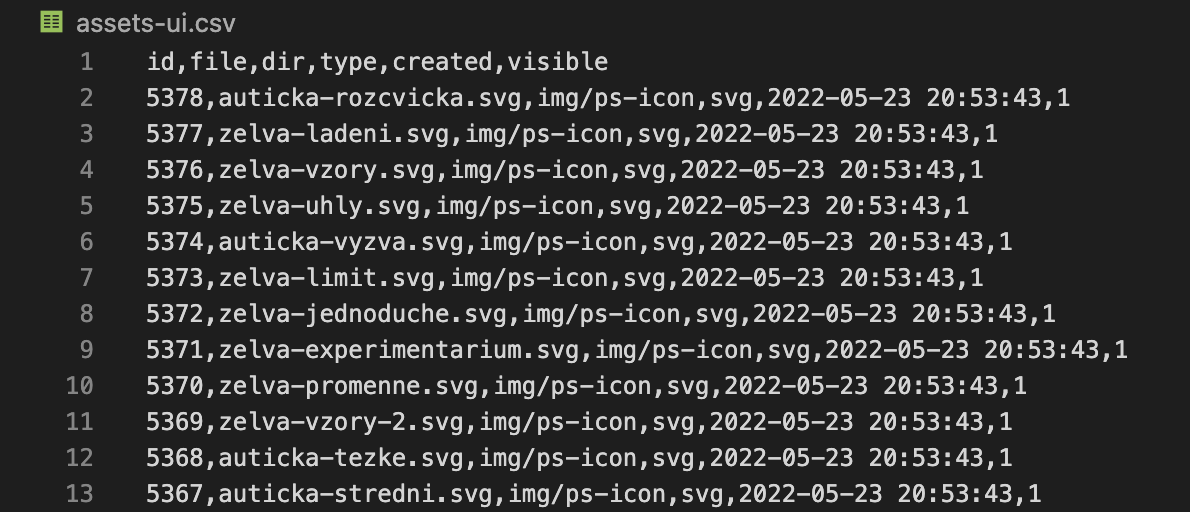
\includegraphics[width=\textwidth]{images/assets-ui-csv.png}
\centering
\caption{First 13 lines of the CSV file for subject Informatics}
\end{figure}

\section{OCR-ing the Images}

With the downloaded images, we can now generate each image's inner text. This step is the most crucial; the data we get from the OCR model must be as accurate as possible.

\section{Working With The OCRed Text}

Here we filter the generated text. Filter out the English words, and keep only the Czech words. The boundary between which words have to be translated is not firmly given, so in this step, we experiment and try different configurations to get the best results.

After the filtering, we get the resulting words found in each image that our model flagged as \emph{should be translated}. We can then generate a list of images that should be translated simply by putting in images with some resulting text associated with them. The images without any text are the ones we don't need to translate.

This list of images is the result of the model.

\chapter{Implementation}\label{chap:implementation}

When implementing the final model I tried many configurations and different tools. In here I try to explain most of the approaches I had when implementing all of the versions, not only the final one.

\section{Python notebooks}

For most of my implementation, I write my code in python notebooks. They do not work like a regular python (.py) file, they work more like R or Matlab scripts. When opened, they initialize their context and then keep that context until closed or restarted.

The code inside these notebooks is divided into code cells, and each code cell can have its output. We can also have markdown cells between code cells for text/explanations.

These notebooks can be created and modified with jupyter~\cite{jupyter}, a python library. Another tool for working with python notebooks from google is Colab\footnote{\href{https://colab.research.google.com/}{https://colab.research.google.com/}}. Both of these editors work in a browser.

For editing and creating python notebooks, I use a VS Code extension that works similarly to the two editors mentioned above.

\textbf{INSERT IMAGE OF THE EDITOR}

\section{Used Tools and Libraries}

\subsection{Pandas}

\emph{\textbf{Pandas} is a fast, powerful, flexible and easy to use open source data analysis and manipulation tool, built on top of the Python programming language.}~\cite{pandas}. With pandas, users can arrange the data inside their DataFrames, similar to DataFrame from the programming language R. These DataFrames are virtual tables with each record stored as a row. Adding, removing, or altering the data within these DataFrames is similar to altering a table in a relational database.

Using pandas is crucial for this thesis, as working with data in python only with the built-in tools would add a lot more work and make the code more cluttered. Also, with pandas visualizing the data is more straightforward, and the visualized data is easier to read.

\begin{figure}[h]
\caption{Example of a visualization of a DataFrame with image path and the OCRed data}
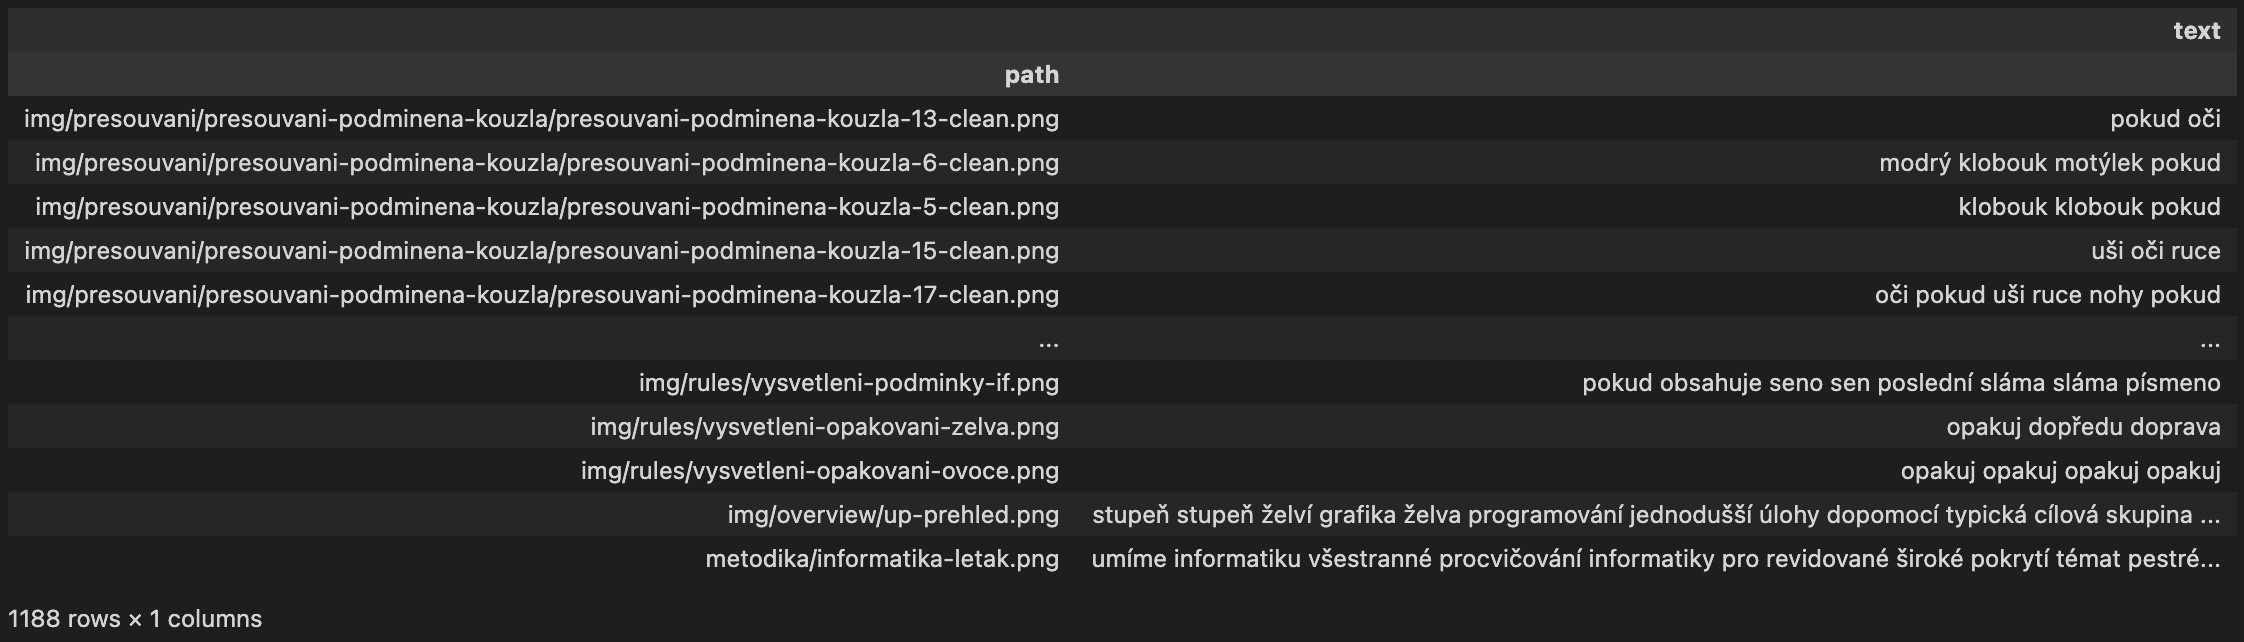
\includegraphics[width=\textwidth]{images/dataframe-visualization.png}
\centering
\end{figure}

\subsection{Numpy}

Numpy~\cite{numpy} is another python library for working with numerical data. Numpy is a core library for data science in python. It implements its arrays (similar to C's arrays) that are more efficient than the built-in data structures of python. Numpy also provides several operations and functions for mathematical structures like matrices or vectors. Since there is not much numerical work involved, I do not depend on this library as much.

\subsection{PIL and Matplotlib}

Since I am working with images, I want to show those images and modify them in preprocessing. For that is the PIL python library. With PIL, we can show the image, change individual pixels, add a margin to an image, and so on.

Since I am working with python notebooks (files with .ipynb extension), I use PIL along with matplotlib, so the image does not open in another window but stays as an output of a given cell.

\subsection{langdetect}

Langdetect is a python wrapper around Shuyo Nakatani's language detection library~\cite{nakatani2010langdetect} implemented in Java. This library claims it has over 99\% precision, which is supported by several test results. Their language detection works especially well with longer texts, but it worked well for this use case.

However, this library is not used in the final model, as just corpus checking was working better.

\section{URL Reconstruction and Images Downloading}

As mentioned in the previous chapter, the input was CSV, from which I can reconstruct the internal path to the image. So the first step is to filter out all the irrelevant assets and create unique paths for each image.

The second step is to prepend each path with the URL to the web, from which we can download the image to our machine.

\begin{minted}{python}
df = pd.read_csv("assets-ui.csv")
df = df[df.type == "image"]

for i, row in df.iterrows():
    url = "https://www.umimeto.org/asset/system/up/" + df["dir"][i] + "/" + df["file"][i]
    local_dir_path = "/data/xvalcik1/ui_images_download/" + df["dir"][i]
    local_img_path = local_dir_path + "/" + df["file"][i]
    print(i, url)
    print(i, local_img_path)
    if os.path.isfile(local_img_path):
        print(i, "already downloaded", end="\n\n")
        continue

    Path(local_dir_path).mkdir(parents=True, exist_ok=True)
    open(local_img_path, 'wb').write(requests.get(url, allow_redirects=True).content)
    print(i, "successfully downloaded", end="\n\n")
\end{minted}

Here, \emph{assets-ui.csv} is the provided CSV file with all the assets used for the subject Informatics. I download all the images to directory \emph{\detokenize{/data/xvalcik1/ui_images_download}} on my local machine.

\section{OCRing The Images}

In the first approach, I use \hyperref[chap:ocr-tesseract]{Tesseract} to get text data of each image. This approach isn't that successful as the generated text often does not correspond to the text inside the images. For improvement, I preprocess the images and then OCR them with Tesseract. Some preprocessing methods bring some better results, but the precision of the OCRed text is still low.

One preprocessing technique I used is adding a white margin to every image.

\begin{minted}{python}
def add_margin(pil_img, color='white'):
    width, height = pil_img.size
    pad_size = width + height
    new_width = width + pad_size
    new_height = height + pad_size
    result = Image.new(pil_img.mode, (new_width, new_height), color)
    result.paste(pil_img, (pad_size // 2, pad_size // 2))
    return result
\end{minted}

This function takes an image as a parameter, adds a margin of a given color (or white if color is not specified), and returns the edited image. The result looks like the figure below.

\begin{figure}[h]
\caption{Image before and after the application of the add\_margin function}
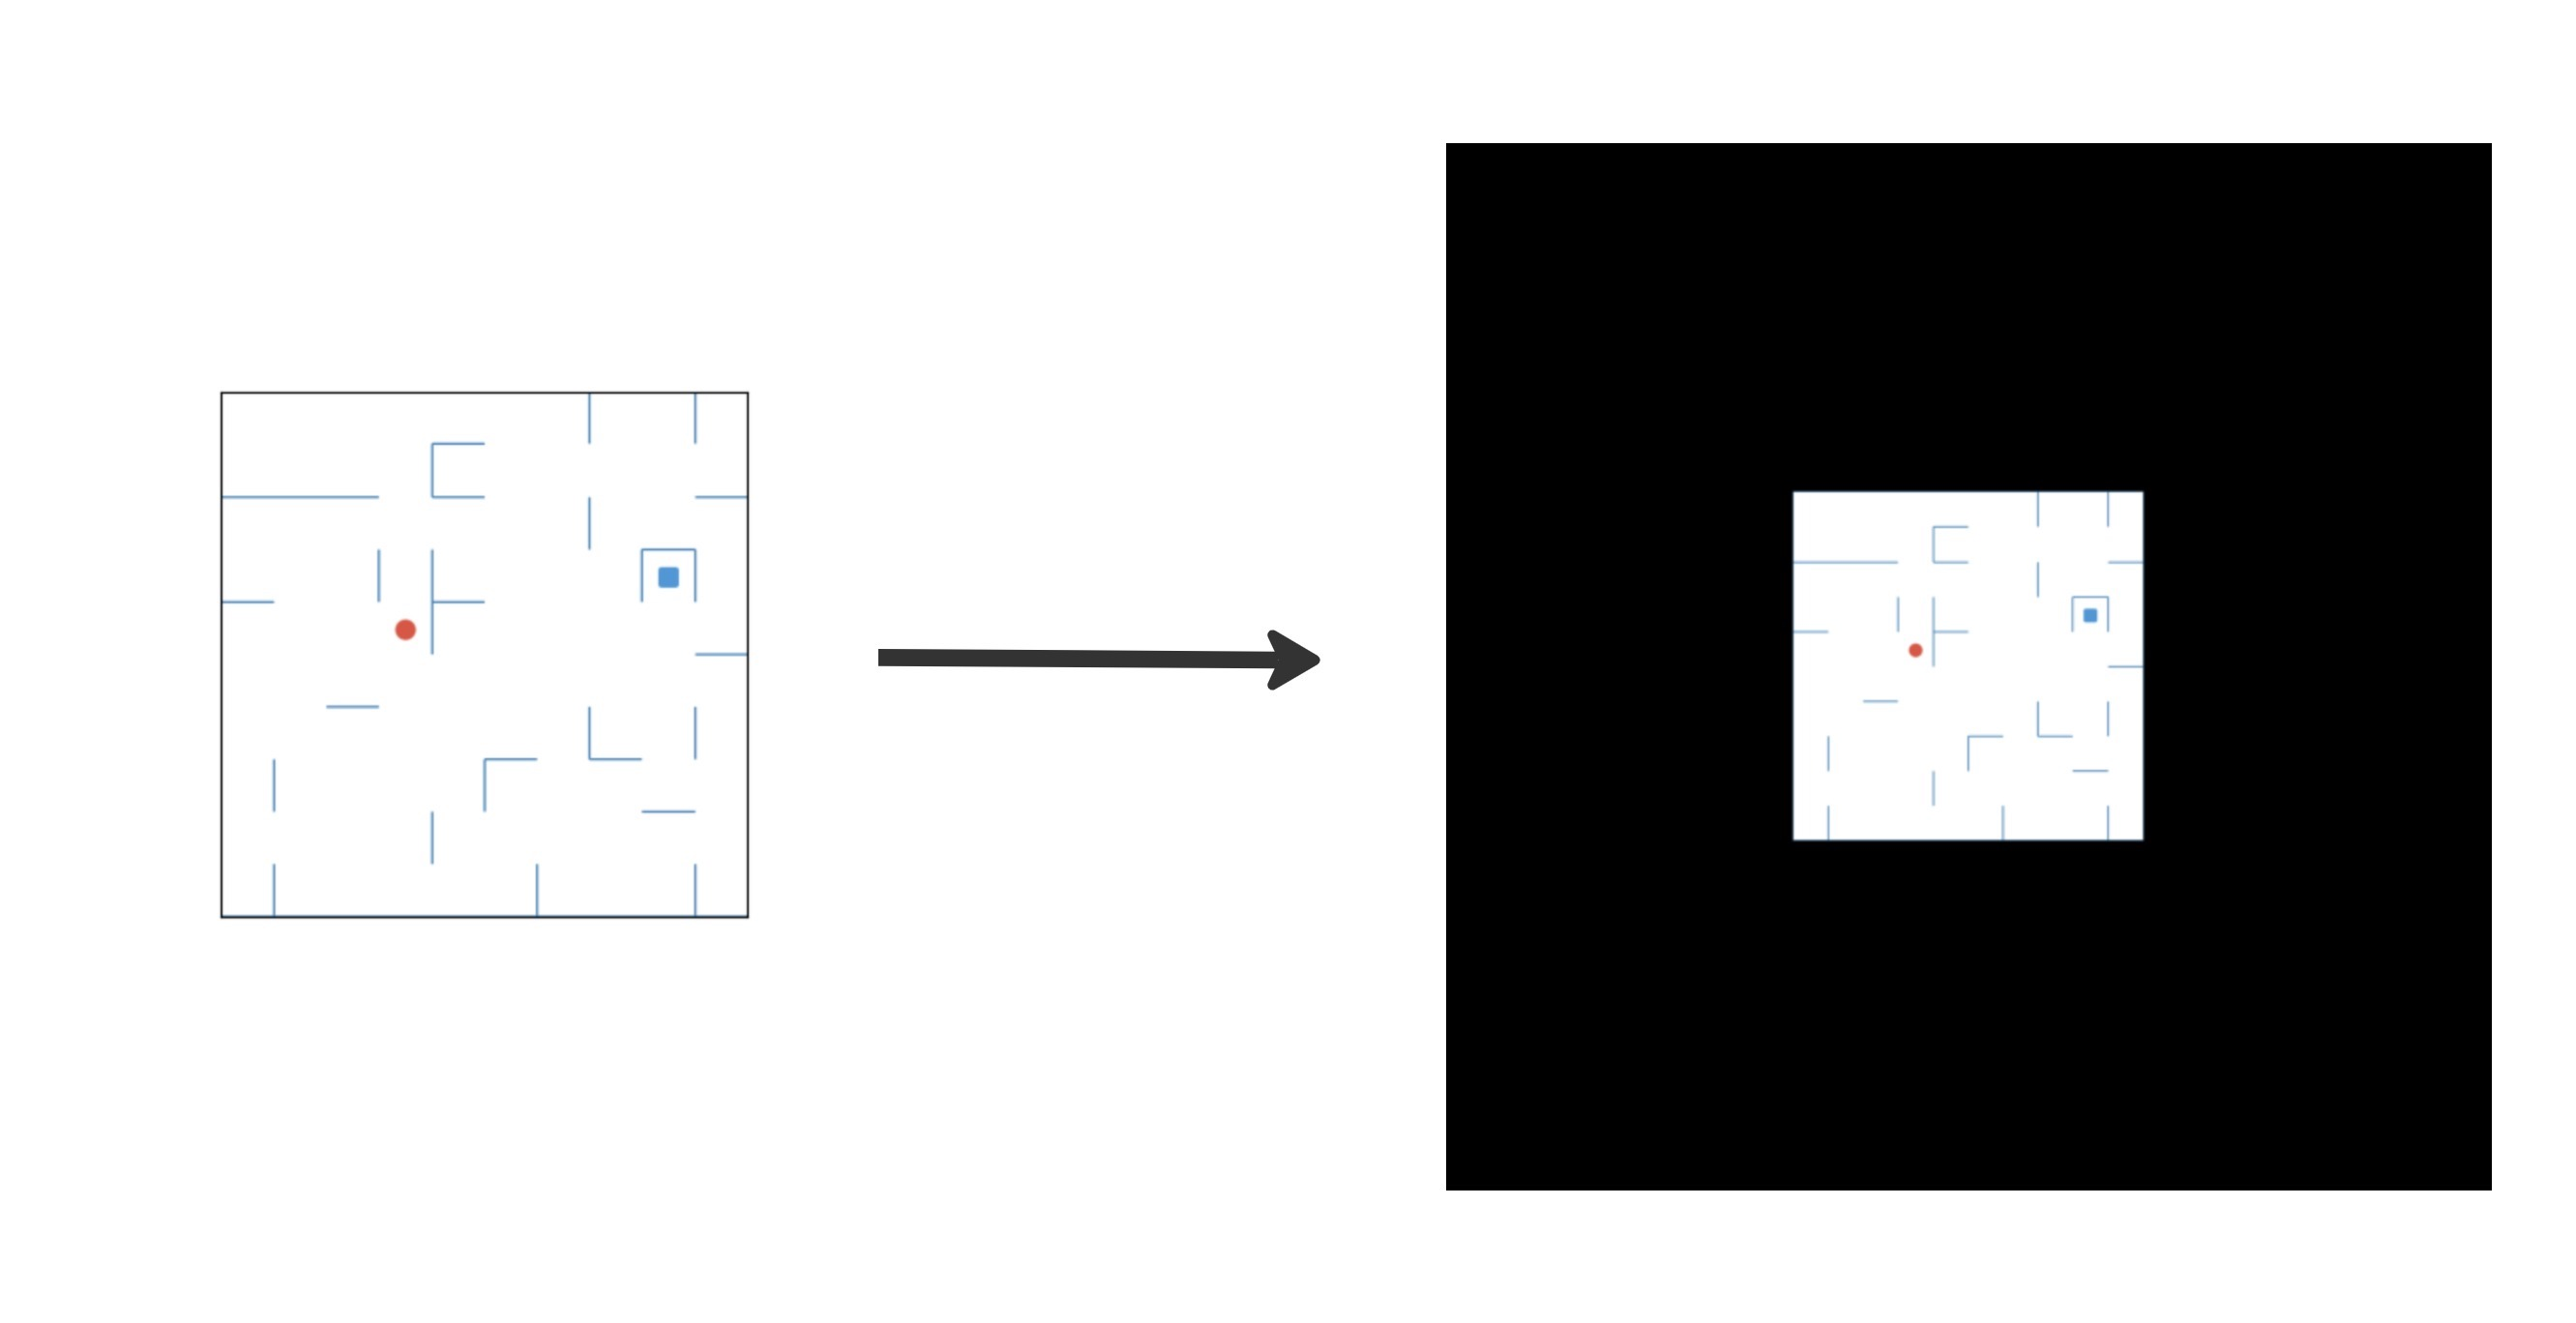
\includegraphics[width=\textwidth]{images/add-margin.jpeg}
\centering
\end{figure}

Another technique I try is thresholding, which converts the image to black and white according to a given threshold.

With either of these preprocessing techniques, I do not achieve any significant improvement with Tesseract.

\textbf{translate this to english}

prvni zpusob byl proste OCRnout images - to nefungovalo uplne nejlepe, tak jsem pridal kazdemu obrazku okraj pomoci funkce \emph{add\_margin(img)} a pak byla uspenost lepsi ale nikoliv super. Jako dalsi check jsem vyuzil slovnikovou kontrolu -> I also added a condition that found word has to have lenght greater of equal to 3, because finding only 2 or 1 char words was adding a lot of false positives (words flagged for translation but without the actual czech text).

Jeste vyuzivam langdetect, ktery dela text -> language, kde primarni zamer byl brat jen ty obrazky, ktere budou detekovane jako cestina, ale nakonec to nebylo uplne stastne (jednoslovne obrazky byly recognized jako jiny slovansky jazyk a to jako jsem dolietal). Ted to pouzival jen tak, ze kdyz je text tak zmateny, ze z toho nejde ani rozpoznat jazyk, tak ho vyhazuji jako beztextovy. In the end I dropped this completely, even for the EasyOCR pipeline.

\subsection{EasyOCR}

For the EasyOCR pipeline, which is also the best performing pipeline on train data, I used the following steps. At first, I basically copied the tesseract pipeline, but in the end, I removed some steps and also added some new steps.

Reconstruct urls from assets-u*.csv file. This is done in the ocr.ipynb notebook, in the first cells. Then I create a new csv file with the corresponding paths of the downloaded images.

Preprocessing: Simple preprocessing was done just by removing the non-image files by looking at the type in the assets-u*.csv and also by looking at the extension of the file. Only after that, I save the paths of the downloaded images to for example \emph{csvs/loaded\_images\_um.csv}.

Run the EasyOCR engine. This is done through the file \emph{easyocr\_run\_all.py}. I separated the actual OCR model into a file because I was running this computation on the Aura computing server, and I needed to set up the \emph{CUDA\_VISIBLE\_DEVICES}, so the computing will be GPU accelerated, and I didn't want to experiment with notebooks, and these settings. This file takes in the \emph{loaded\_images\_u*.csv} and returns another CSV with the OCRed words along with other metadata. A sample output of one image is below. The file generated from this step is for example \emph{csvs/easyocr/um\_trainset.csv} (which is the assets-um.csv OCRed).

\begin{verbatim}
    0,/data/xvalcik1/ui\_images\_download/img/presouvani/presouvani-podminena-kouzla/presouvani-podminena-kouzla-10-clean.png,"[([[659, 141], [1040, 141], [1040, 242], [659, 242]], 'pokud 2 ruce:', 0.9814824196590307), ([[1263, 140], [1646, 140], [1646, 242], [1263, 242]], 'pokud 2 ruce:', 0.8691733092857169), ([[726, 241], [1008, 241], [1008, 329], [726, 329]], 'Kloboukuj', 0.890718448642362), ([[1328, 233], [1615, 233], [1615, 333], [1328, 333]], 'Kloboukuj', 0.9472866960821049), ([[725, 337], [979, 337], [979, 423], [725, 423]], 'motýlkuj', 0.9982528021469238), ([[1273, 337], [1527, 337], [1527, 423], [1273, 423]], 'motýlkuj', 0.9986867684056133)]"
\end{verbatim}




All the steps done now can be viewed in the file pipeline.ipynb in the first code cell. Basically, the steps were as such:

Extract just words from the outputs [([[659, 141], [1040, 141], [1040, 242], [659, 242]], 'pokud 2 ruce:', 0.9814824196590307), ([[1263, 140], [1646, 140], [1646, 242], [1263, 242]], 'pokud 2 ruce:', 0.8691733092857169) -> pokud 2 ruce: pokud 2 ruce:

Doing a Czech language dictionary check -> leave in only words that are also in the syn2015 Czech corpus. This actually wasn't as useful as I thought it was going to be, because there are A LOT of words in the Czech corpus.
Getting only words with len >= 3

Remove English words. I downloaded a corpus of English words (\emph{slovnik/english\_dict.csv}) and if a found word was also present in the English corpus, I removed that word. This could be the most problematic step, maybe I could investigate it.

\section{Problematic cases}

In here I'll discuss some interesting cases that were causing problems.

\chapter{Evaluation}\label{chap:evaluation}

So far I've only done a simple evaluation that went like this. This procedure was the same for all the evaluations done so far:

We have a set of images, we run the OCR pipeline and we end up with a .csv file with two columns, first one is the path and the second one is the words that are considered to be present in the image. So the final .csv contains all the images flagged as positives, and if we do a set difference between the original set of images and the flagged images, we get the negatives.

I did checks for false negatives and for false positives. They both went similarly. First I'd sample 100 images from one of the classes (positives or negatives), and then I'd look at the images and write the paths down if they were either a false-positive or false-negative. That's how I could really roughly estimate the percentages of both these false classes.

\subsection{Evaluation of the test set on the current EasyOCR pipeline}

With the evaluation procedure mentioned above, I evaluated the testset provided. The test set is all the images used for Umíme informatiku, that being 5256 images in total. After running the pipeline I ended up with 1188 images flagged as positive, meaning around 22.6\% of the images were flagged as having Czech text in them.
Then I evaluated false positives/negatives.

\subsubsection{False positives}
None of the images was marked as false positive. Every image flagged as positive was indeed positive (had Czech text in it).

\subsubsection{False negatives}
With false negatives, this was quite worse. 18/100 were flagged as a false negative. This sums up to "only" to about 18\% of the false-negative rate, but when only around 22\% of images from the whole dataset were flagged as positive, that 18\% is actually pretty big. If we indeed had 18\% of images flagged as negative being actually positive, we missed almost half of the truly positive images in the dataset.

\chapter{Conclusion}

\end{document}
